\documentclass[11pt,a4paper]{article}

% =============================================
% Paquetes
% =============================================
\usepackage[utf8]{inputenc}
\usepackage[T1]{fontenc}
\usepackage[spanish,es-tabla]{babel}
\usepackage{amsmath,amssymb}
\usepackage{graphicx}
\usepackage{booktabs}
\usepackage{enumitem}
\usepackage{geometry}
\usepackage{setspace}
\usepackage{hyperref}
\usepackage[numbers]{natbib}
\usepackage{xcolor}
\usepackage{fancyhdr}
\usepackage{titlesec}
\usepackage{float}
\usepackage{caption}
\usepackage{tcolorbox}
\usepackage{tabularx}
\usepackage{array}
\usepackage{url}
\urlstyle{tt}

% Public repository (GitHub; Zenodo DOI filled at archival release)
\newcommand{\ExcessThreeRepo}{https://github.com/johelpadilla/excess3}
\newcommand{\ExcessThreeRepoShort}{github.com/johelpadilla/excess3}
% \newcommand{\ExcessThreeDOI}{10.5281/zenodo.XXXXXXX}  % set at Zenodo release

\geometry{margin=1.05in}
\onehalfspacing
\setlist[itemize]{itemsep=4pt,topsep=4pt}
\setlist[enumerate]{itemsep=4pt,topsep=4pt}

\titleformat{\section}{\large\bfseries}{\thesection}{0.6em}{}
\titleformat{\subsection}{\normalsize\bfseries}{\thesubsection}{0.5em}{}
\titleformat{\subsubsection}{\normalsize\itshape}{\thesubsubsection}{0.5em}{}

\pagestyle{fancy}
\fancyhf{}
\fancyhead[L]{\small excess$^3$: dependencia de orden 3}
\fancyhead[R]{\small \thepage}
\renewcommand{\headrulewidth}{0.4pt}

\hypersetup{
  colorlinks=true,
  linkcolor=blue!60!black,
  citecolor=blue!60!black,
  urlcolor=blue!70!black,
  pdftitle={excess3: dependencia de orden 3 y surplus sinérgico},
  pdfauthor={Johel Padilla-Villanueva},
  pdfkeywords={excess3, sinergia, dependencia multivariada, sistemas complejos}
}

% Figuras y macros numéricos del preprint de métodos
\graphicspath{{../methods/figures/}}
% Auto-generated by scripts/fill_numbers_from_json.py — do not edit by hand
\newcommand{\NumT}{1000}
\newcommand{\NumEvent}{500}
\newcommand{\NumR}{25}
\newcommand{\NumB}{99}

% G0
\newcommand{\GzeroPre}{1.8331}
\newcommand{\GzeroPost}{1.8358}
\newcommand{\GzeroDelta}{+0.0028}
\newcommand{\GzeroMedP}{0.560}
\newcommand{\GzeroFrac}{4\%}
\newcommand{\GzeroOccPost}{1.000}

% G1
\newcommand{\GonePre}{1.8308}
\newcommand{\GonePost}{1.7332}
\newcommand{\GoneDelta}{-0.0977}
\newcommand{\GoneMedP}{0.010}
\newcommand{\GoneFrac}{92\%}
\newcommand{\GoneOccPost}{1.000}

% G2
\newcommand{\GtwoPre}{1.6273}
\newcommand{\GtwoPost}{1.6192}
\newcommand{\GtwoDelta}{-0.0081}
\newcommand{\GtwoMedP}{0.510}
\newcommand{\GtwoFrac}{8\%}
\newcommand{\GtwoOccPost}{1.000}

% G3
\newcommand{\GthreePre}{1.8374}
\newcommand{\GthreePost}{1.7893}
\newcommand{\GthreeDelta}{-0.0482}
\newcommand{\GthreeMedP}{0.080}
\newcommand{\GthreeFrac}{40\%}
\newcommand{\GthreeOccPost}{1.000}



\newtcolorbox{idea}[1][]{
  colback=blue!4!white, colframe=blue!70!black,
  title={\textbf{Idea clave}}, fonttitle=\bfseries,
  boxrule=0.7pt, left=5pt, right=5pt, top=3pt, bottom=3pt, #1
}
\newtcolorbox{atencion}[1][]{
  colback=orange!6!white, colframe=orange!70!black,
  title={\textbf{Precauci\'on}}, fonttitle=\bfseries,
  boxrule=0.7pt, left=5pt, right=5pt, top=3pt, bottom=3pt, #1
}

\title{\textbf{excess$^3$: dependencia de orden 3\\
y surplus sin\'ergico en sistemas multivariados}\\[0.45em]
\large Motivaci\'on, construcci\'on, lectura, validaci\'on sint\'etica\\
e interpretaci\'on}

\author{
Johel Padilla-Villanueva \\
\textit{Departamento de Salud Ambiental, Universidad de Puerto Rico} \\
ORCID: \href{https://orcid.org/0000-0002-5797-6931}{0000-0002-5797-6931} \\
\texttt{johelpadilla@gmail.com} \\
\texttt{joel.padilla2@upr.edu}
}

\date{Preprint v1.0 \quad | \quad julio 2026 \\[0.25em]\small Repositorio: \href{\ExcessThreeRepo}{\ExcessThreeRepoShort}}

\begin{document}
\maketitle

% =============================================
\begin{abstract}
\noindent
En muchos sistemas medidos a lo largo del tiempo, tres o m\'as variables
pueden reorganizarse de manera conjunta sin que ninguna de ellas, por
separado, se vuelva extrema, y sin que las relaciones de a dos basten para
describir lo que ocurre. Ese fen\'omeno se denomina aqu\'i
\textbf{dependencia de orden 3} o, en sentido operativo,
\textbf{surplus sin\'ergico}: organizaci\'on residual del conjunto que no se
agota en las interacciones por pares.

La medida \textbf{excess$^3$} (en software, \texttt{excess3}) cuantifica ese
sobrante combinando dos componentes complementarios. El primero,
$\mathrm{Syn}$, es el residual de multiinformaci\'on que permanece despu\'es
de restar una baseline construida con informaciones mutuas de a pares. El
segundo, $\mathrm{Surp}$, mide cu\'anto m\'as frecuentes son ciertas
combinaciones conjuntas de s\'imbolos respecto de lo que esperar\'ia un
modelo de independencia completa entre canales. Ambos se agregan con pesos
fijos $0.6/0.4$, elegidos a priori. El resultado es un puntaje continuo por
ventana de tiempo; el contraste $\Delta\mathrm{excess3}$ y las pruebas con
surrogados de barajado de fase permiten evaluar cambios de r\'egimen sin
convertir el n\'umero en una tesis causal ni en un \'atomo completo de
descomposici\'on parcial de informaci\'on (PID).

Bajo hiperpar\'ametros de referencia ($m=3$, $w=13$, pesos $0.6/0.4$) y un
dise\~no con $R=\NumR$ realizaciones, $B=\NumB$ surrogados y series de
longitud $T=\NumT$, la validaci\'on sint\'etica en cuatro brazos se comporta
de forma coherente con las predicciones de dise\~no. El brazo casi nulo de
canales AR(1) independientes (G0) produce media
$\Delta=\GzeroDelta$ y mediana $p=\GzeroMedP$ ($\GzeroFrac$ de
realizaciones con $p<0.05$). El brazo de reorganizaci\'on plantada por
latente compartido (G1) produce media $\Delta=\GoneDelta$, mediana
$p=\GoneMedP$ y $\GoneFrac$ de realizaciones extremas a dos colas; el signo
negativo es informativo porque el acoplamiento com\'un infla la baseline de
parejas y puede reducir el residual Syn. El mapa log\'istico acoplado (G2)
queda cerca del nulo en este dise\~no (media $\Delta=\GtwoDelta$), y el
control solo de a pares (G3) es intermedio (media $\Delta=\GthreeDelta$,
mediana $p=\GthreeMedP$). A $\theta_3=0.08$, la ocupaci\'on de $\Phi_3$ se
satura; la discriminaci\'on vive en el $\Delta$ continuo.

El presente trabajo motiva la medida con ejemplos, introduce el vocabulario
de incertidumbre e informaci\'on compartida, construye excess$^3$ con un
c\'alculo num\'erico tipo XOR, integra las figuras y hallazgos del protocolo
sint\'etico, y delimita lo que la medida no afirma. La definici\'on can\'onica,
el protocolo de nulos y el checklist de reporte est\'an en el preprint de
m\'etodos \citep{Padilla2026excess3}; este texto desarrolla motivaci\'on,
lectura e interpretaci\'on con evidencia, sin redefinir el estad\'istico. El
marco Systemic Tau / RECD se cita donde orienta el uso de Level~3
\citep{Padilla2026framework}.
\end{abstract}

\noindent\textbf{Palabras clave:}
excess$^3$, dependencia multivariada, sinergia, multiinformaci\'on,
sistemas complejos, patrones ordinales, surrogados, validaci\'on sint\'etica

\vspace{0.35cm}

\begin{idea}
excess$^3$ mide organizaci\'on entre tres o m\'as variables que no se reduce
a mirarlas de dos en dos. Devuelve un n\'umero continuo por ventana y se
contrasta con un modelo nulo sobre el estad\'istico completo (por ejemplo
$|\Delta\mathrm{excess3}|$). Por s\'i sola no produce una historia causal ni
una prueba de emergencia metaf\'isica.
\end{idea}

\tableofcontents
\newpage

% =============================================
\section{Organizaci\'on del trabajo}
\label{sec:como}

El argumento se desarrolla de lo concreto a lo formal y de lo formal a la
evidencia sint\'etica y a la pr\'actica. Primero se motiva, con ejemplos, por
qu\'e la reorganizaci\'on conjunta puede ser invisible para las herramientas
que solo miran parejas (secciones~\ref{sec:historia}--\ref{sec:xor_idea}).
Despu\'es se introduce el vocabulario de incertidumbre e informaci\'on
compartida (secci\'on~\ref{sec:entropia}), la codificaci\'on ordinal
(secci\'on~\ref{sec:simbolos}) y la construcci\'on de excess$^3$, con un
c\'alculo num\'erico completo en geometr\'ia XOR
(secciones~\ref{sec:piezas}--\ref{sec:xor}). Las secciones siguientes tratan
la lectura de magnitudes, los l\'imites de interpretaci\'on y el protocolo de
nulos (secciones~\ref{sec:leer}--\ref{sec:nulos}). La
secci\'on~\ref{sec:validation} integra el dise\~no G0--G3, las tablas de
resultados y las seis figuras del protocolo sint\'etico de referencia. El
cierre sit\'ua la medida en Systemic Tau / RECD, esboza usos por dominio y
propone un flujo de an\'alisis (secciones~\ref{sec:recd}--\ref{sec:flujo}).
La secci\'on~\ref{sec:diseno} consolida seis decisiones de dise\~no que
suelen generar confusi\'on en la lectura aplicada (pesos, Syn frente a Surp,
primac\'ia del continuo, alcance PID, nulos y anidamiento). Los detalles de
implementaci\'on y de software se remiten a \citep{Padilla2026excess3}.

\begin{idea}
\textbf{Jerarqu\'ia de la familia.} El preprint de m\'etodos
\citep{Padilla2026excess3} \emph{define} el contrato (ecuaciones, nulos,
validaci\'on, checklist). Este trabajo \emph{motiva y lee} ese contrato en
espa\~nol, con figuras y n\'umeros del mismo protocolo. La gu\'ia
interdisciplinaria en ingl\'es \citep{Padilla2026primer} \emph{ense\~na} el
uso prudente (analog\'ias, vi\~netas de dominio, notas de taller). Las tres
piezas no compiten: solo el methods es citaci\'on can\'onica de
implementaci\'on.
\end{idea}

% =============================================
\section{Motivaci\'on: reorganizaci\'on conjunta}
\label{sec:historia}

\subsection{Monitoreo fisiol\'ogico}

Consid\'erese un entorno cl\'inico en el que se registran de forma simult\'anea
tres se\~nales de un paciente cr\'itico: el patr\'on del ritmo card\'iaco
($A$), el de la respiraci\'on ($B$) y el de la presi\'on arterial ($C$). En
muchas jornadas cl\'inicas, ninguna de las tres cruce por s\'i sola un umbral
de alarma. Las lecturas univariadas parecen ``dentro de rango'', y sin
embargo un observador experimentado puede notar que el sistema dej\'o de
coordinarse como lo hac\'ia horas antes. La intuici\'on no habla del tama\~no
absoluto de cada canal, sino de la \emph{organizaci\'on entre} canales: de
c\'omo se entrelazan en el tiempo. Esa intuici\'on es relacional. excess$^3$
intenta convertir una intuici\'on de ese tipo en un n\'umero reproducible,
con un procedimiento fijo y con un contraste frente a un mundo nulo, sin
pretender que el n\'umero agote el juicio cl\'inico ni demuestre un mecanismo
fisiol\'ogico concreto.

\subsection{Clima, vector e incidencia}

Un segundo escenario, de salud ambiental, ilustra el mismo punto con otra
vestimenta. Sean tres series diarias en una regi\'on: lluvia, densidad de
mosquitos y casos de fiebre. Es perfectamente posible que la lluvia, tomada
sola, prediga poco la incidencia, y que la densidad de mosquitos, tomada
sola, tampoco baste. Aun as\'i, la combinaci\'on ``lluvia reciente y
mosquitos elevados'' puede asociarse de modo mucho m\'as claro con lo que
viene despu\'es. Un an\'alisis que solo calcule correlaciones o informaciones
mutuas de a pares puede subestimar el fen\'omeno, porque la estructura
relevante no vive en las aristas del grafo bivariado, sino en la ley
conjunta de las tres variables. Cuando se mira el tr\'io, aparece una
organizaci\'on de conjunto que las parejas, aisladas, diluyen o disimulan.

\subsection{Dos geometr\'ias distintas de ``las tres se mueven''}

No toda co-movilizaci\'on de tres variables es del mismo tipo. Una caja
fuerte que exige tres llaves a la vez ilustra lo que se llamar\'a
\emph{sinergia de orden 3} en sentido informal: cualquier par de llaves es
insuficiente; solo el tr\'io es decisivo. Una caja con una sola llave maestra
que abre tres cerraduras ilustra, en cambio, una geometr\'ia m\'as cercana a
la \emph{redundancia} o al conductor com\'un: las parejas se ven
fuertemente relacionadas precisamente porque comparten la misma llave. En
el primer caso, las herramientas de a pares pueden quedar casi ciegas; en
el segundo, brillan. excess$^3$ est\'a dise\~nado para ser sensible, sobre
todo, al sobrante que queda cuando las parejas no agotan la organizaci\'on
conjunta, aunque en datos reales ambas geometr\'ias se mezclan y el signo
de un contraste puede reflejar esa mezcla de maneras no triviales, como se
ver\'a en la validaci\'on sint\'etica del brazo G1.

\begin{idea}
Hay, al menos, dos mundos distintos. En el mundo de parejas, casi todo lo
relevante se ve mirando de dos en dos. En el mundo de tr\'io, hay
organizaci\'on que solo aparece cuando las tres variables se consideran
juntas. excess$^3$ se orienta al segundo, mediante un dise\~no h\'ibrido que
combina residual multiinformacional y sorpresa de independencia.
\end{idea}

% =============================================
\section{Variables, dependencia y el l\'imite de las parejas}
\label{sec:cero}

Una variable, en este trabajo, es simplemente una cantidad observada a lo
largo del tiempo: temperatura, n\'umero de casos, ritmo card\'iaco, precio,
conteo de una especie, un \'indice clim\'atico o un biomarcador. Cuando se
registran varias a la vez, se tiene un sistema multivariado. Dos variables
dependen en sentido estad\'istico si el conocimiento de una reduce la
incertidumbre sobre la otra. Si siempre que llueve mucho sube el r\'io,
lluvia y nivel del r\'io dependen. Si el color de una camisa y el precio del
caf\'e en otra ciudad no se relacionan de modo sistem\'atico, son
pr\'acticamente independientes bajo el estimador empleado.

Es crucial no confundir dependencia estad\'istica con causaci\'on. Dos
relojes pueden marcar la misma hora sin que uno cause al otro; ambos pueden
estar sincronizados por un tercero ---la red el\'ectrica, un servidor de
tiempo, un ritmo estacional---. excess$^3$ habla de co-organizaci\'on bajo un
c\'odigo y una ventana, no de flechas de mecanismo. Esa distinci\'on debe
permanecer visible en la redacci\'on de resultados.

Las herramientas m\'as comunes de la pr\'actica cient\'ifica miran parejas:
correlaciones de Pearson o Spearman, informaci\'on mutua bivariada, redes en
las que cada arista representa una relaci\'on significativa entre dos nodos.
Son herramientas excelentes y, en muchos problemas, suficientes. Su
limitaci\'on no es un defecto moral, sino un l\'imite de orden: responden a
la pregunta de c\'omo se relacionan dos variables y no agotan la pregunta de
si hay estructura que solo se ve cuando tres o m\'as se consideran
conjuntamente. El candado XOR es el prototipo cl\'asico de esa limitaci\'on.

La tabla~\ref{tab:compare} sit\'ua excess$^3$ respecto de medidas
relacionadas que el lector interdisciplinario suele invocar. La informaci\'on
de interacci\'on puede ser negativa y captura una interacci\'on de tr\'iple
firmada; la O-informaci\'on descompone modos globales de redundancia frente a
sinergia; el \'atomo sin\'ergico de PID es el objetivo conceptual m\'as puro y
tambi\'en el m\'as exigente en muestra y estabilidad
\citep{Williams2010,Rosas2019,McGill1954}. excess$^3$ no pretende
reemplazarlos: es un proxy pre-especificado y computable cuando se necesita
un contraste continuo de surplus de orden 3 alineado con un pipeline de
software \citep{Padilla2026excess3}.

\begin{table}[H]
\centering
\caption{Posicionamiento de excess$^3$ respecto a medidas multivariadas
relacionadas.}
\label{tab:compare}
\small
\begin{tabularx}{\textwidth}{@{}>{\raggedright\arraybackslash}p{2.8cm}
  >{\raggedright\arraybackslash}X
  >{\raggedright\arraybackslash}p{1.7cm}
  >{\raggedright\arraybackslash}X@{}}
\toprule
\textbf{Medida} & \textbf{Qu\'e captura} & \textbf{Costo} &
\textbf{Relaci\'on con excess$^3$} \\
\midrule
Informaci\'on de interacci\'on $I(X;Y;Z)$
  & Sinergia $+$ redundancia (puede ser negativa)
  & Bajo
  & Prima conceptual; excess$^3$ busca un surplus residual no negativo \\
O-informaci\'on / S-informaci\'on
  & Descomposici\'on global redundancia vs.\ sinergia
  & Medio
  & M\'as global; no fijada a orden exactamente 3 \\
\'Atomo sin\'ergico PID
  & Sinergia at\'omica del lattice
  & Alto
  & Objetivo conceptual; excess$^3$ es proxy cuando PID estable no es factible \\
\textbf{excess$^3$}
  & Surplus sin\'ergico h\'ibrido de orden 3
  & Bajo--med.
  & Proxy continuo pre-especificado con pesos $0.6/0.4$ \\
\bottomrule
\end{tabularx}
\end{table}

% =============================================
\section{El candado XOR como prototipo de orden 3}
\label{sec:xor_idea}

Consid\'erense dos monedas justas, $A$ y $B$, con valores $0$ y $1$, y
def\'inase una tercera variable $C$ que vale $1$ cuando $A$ y $B$ son
distintas y $0$ cuando son iguales. En lenguaje corriente, $C$ es el bit de
``¿son diferentes?''; en \'algebra, es la operaci\'on XOR. Si se examina solo
el par $(A,C)$, a veces coinciden y a veces no, y en promedio $A$ no predice
$C$. Lo mismo ocurre con $(B,C)$. El par $(A,B)$ es, por construcci\'on, de
monedas independientes. Un an\'alisis que solo dibuje un grafo de aristas
bivariadas concluir\'a, de forma enga\~nosa, que no hay relaciones.

La conclusi\'on cambia por completo cuando se mira el tr\'io. Conocer $A$ y
$B$ determina $C$ con certeza. El sistema est\'a fuertemente organizado a
nivel de tres variables, aunque cada pareja, aislada, se vea vac\'ia. Ese es
el prototipo mental de la sinergia de orden 3 en sentido informal: las
partes de a dos no cuentan la historia; el conjunto s\'i. La distinci\'on
operativa frente al conductor com\'un queda entonces clara. Cuando las tres
variables suben juntas porque comparten un factor com\'un, las parejas se
ven fuertes. Cuando la tercera es funci\'on de las dos primeras al estilo
XOR, las parejas se ven d\'ebiles y el tr\'io, fuerte. excess$^3$ se orienta
sobre todo a detectar y cuantificar el segundo tipo de organizaci\'on, sin
negar que en series reales ambos reg\'imenes se superponen.

% =============================================
\section{De la met\'afora al estad\'istico}
\label{sec:numero}

Las met\'aforas organizan el pensamiento, pero un estudio cient\'ifico
necesita un procedimiento reproducible, un n\'umero comparable a lo largo
del tiempo y una forma de preguntar si el contraste observado podr\'ia
aparecer bajo un proceso que conserve rasgos univariados y rompa la
organizaci\'on cruzada. excess$^3$ responde a esas tres exigencias de modo
deliberadamente modesto. En cada ventana de tiempo se calcula un puntaje
continuo $\mathrm{excess3}(t)$. Entre dos reg\'imenes ---antes y despu\'es de
un evento, condici\'on A frente a condici\'on B--- se forma el contraste
$\Delta\mathrm{excess3}$. Ese contraste se sit\'ua despu\'es en una nube de
valores obtenidos bajo un modelo nulo, por ejemplo mediante surrogados que
barajan la fase de cada se\~nal.

\begin{atencion}
Un valor alto de excess$^3$ no significa, por s\'i solo, que se haya
encontrado la causa de un fen\'omeno, que exista ``emergencia fuerte'' en
sentido filos\'ofico, ni que el sistema posea propiedades que el n\'umero no
mide. La lectura honesta es m\'as estrecha y m\'as \'util: bajo el c\'odigo
simb\'olico elegido y dentro de la ventana de estimaci\'on, hay m\'as sobrante
de organizaci\'on conjunta del que explicar\'ian, por un lado, las
interacciones de a pares y, por otro, un modelo de independencia completa
entre canales.
\end{atencion}

% =============================================
\section{Incertidumbre e informaci\'on compartida}
\label{sec:entropia}

La construcci\'on de excess$^3$ se apoya en tres nociones cl\'asicas de la
teor\'ia de la informaci\'on. La \textbf{entrop\'ia} $H(X)$ mide la
incertidumbre de una variable. En bits, una moneda justa tiene entrop\'ia $1$
y una moneda que siempre sale cara tiene entrop\'ia $0$. La regla operativa
es simple: cuanto m\'as impredecible es la variable bajo la distribuci\'on
estimada, mayor es su entrop\'ia. En la pr\'actica de excess$^3$, esas
entrop\'ias se estiman sobre s\'imbolos observados en una ventana.

La \textbf{informaci\'on mutua} $I(X;Y)$ mide cu\'anto se relacionan dos
variables en t\'erminos de incertidumbre compartida. Si son independientes
bajo la distribuci\'on estimada, $I(X;Y)=0$. Si conocer la lluvia reduce de
modo sustancial la incertidumbre sobre el nivel del r\'io, la informaci\'on
mutua es grande; si no aporta nada, se acerca a cero. Constituye el ladrillo
con el que se construye la baseline de parejas.

La \textbf{correlaci\'on total} o \textbf{multiinformaci\'on}, denotada TC,
extiende la idea al conjunto de $N$ variables:
\begin{equation}
\mathrm{TC}(X_1,\ldots,X_N)
=
\sum_{i=1}^{N}H(X_i)-H(X_1,\ldots,X_N).
\end{equation}
TC vale cero solo bajo independencia mutua completa. Una TC alta indica que
el conjunto est\'a organizado muy por encima del producto de las marginales,
pero no dice, por s\'i sola, si esa organizaci\'on es sobre todo de orden 2
o de orden superior.

El movimiento conceptual de excess$^3$ consiste en preguntar cu\'anto sobra
de organizaci\'on despu\'es de restar lo que ya explican las parejas. La
baseline empleada escala la media de las informaciones mutuas bivariadas de
modo que sea comparable con TC:
\begin{equation}
I_{\mathrm{pair}}
=
(N-1)\cdot\overline{I}_{ij},
\end{equation}
donde $\overline{I}_{ij}$ es el promedio de $I(X_i;X_j)$ sobre los pares
\citep{Padilla2026framework,Padilla2026excess3}. El residual no negativo
\begin{equation}
\mathrm{Syn}
=
\bigl[\mathrm{TC}-I_{\mathrm{pair}}\bigr]_+
=
\max\{\mathrm{TC}-I_{\mathrm{pair}},0\}
\end{equation}
es grande cuando la multiinformaci\'on supera de forma clara lo que las
parejas ya cuentan, y se colapsa hacia cero cuando las parejas absorben
casi toda la organizaci\'on conjunta.

A ese residual se a\~nade una segunda pregunta, de geometr\'ia distinta:
¿aparecen combinaciones conjuntas de s\'imbolos m\'as a menudo de lo que
permitir\'ia el producto de las marginales? Esa es la
\textbf{sorpresa de independencia} $\mathrm{Surp}$, una suma ponderada de
log-razones positivas entre la frecuencia emp\'irica de cada tupla conjunta
y la frecuencia que tendr\'ia bajo independencia completa. La medida h\'ibrida
\begin{equation}
\label{eq:excess3}
\mathrm{excess3}
=
0.6\,\mathrm{Syn}
+
0.4\,\mathrm{Surp}
\end{equation}
las combina con pesos fijos. Esos pesos se eligen a priori y forman parte
del objeto metodol\'ogico: no se retocan sobre el mismo dataset con el que
despu\'es se reclama el hallazgo principal.

\begin{idea}
excess$^3$ es un promedio ponderado fijo de dos lentes. $\mathrm{Syn}$
pregunta qu\'e sobra despu\'es de restar parejas; $\mathrm{Surp}$ pregunta
cu\'an sorprendentes son las combinaciones conjuntas frente a la
independencia. El h\'ibrido es un proxy computable de surplus de orden 3,
no un veredicto PID completo.
\end{idea}

La figura~\ref{fig:schematic} resume el flujo completo, desde la serie
multivariada hasta el continuo y el tic binario opcional.

\begin{figure}[H]
\centering
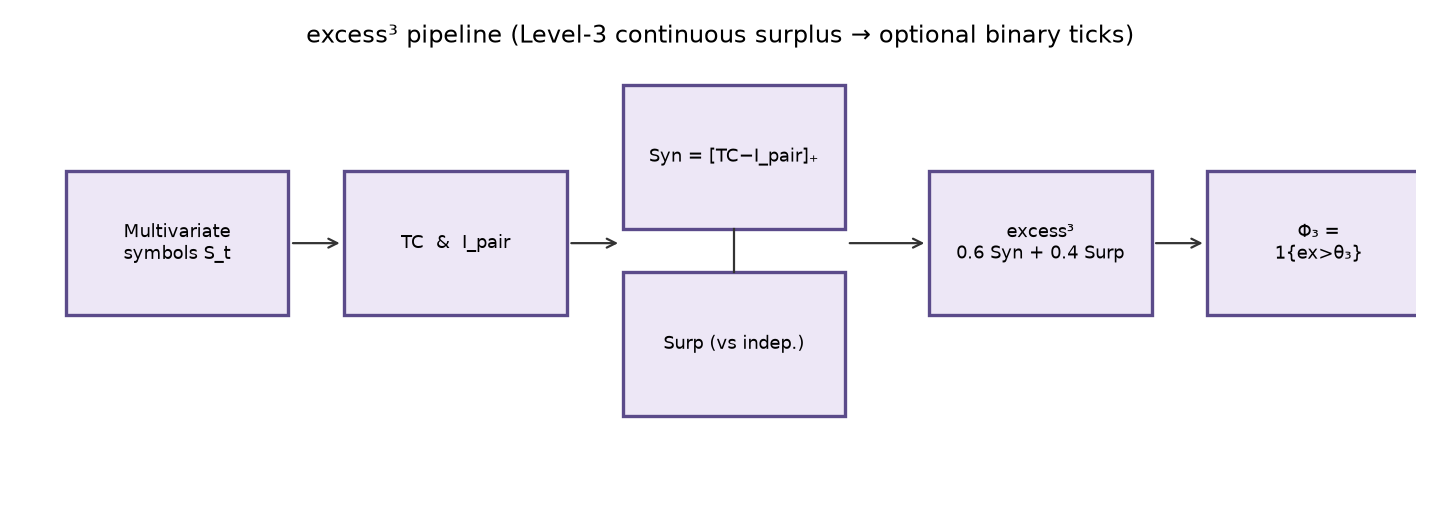
\includegraphics[width=\textwidth]{fig1_schematic.png}
\caption{Flujo conceptual y num\'erico de excess$^3$. Las series
multivariadas se codifican como s\'imbolos ordinales Bandt--Pompe $S_t$;
en cada ventana se estiman la correlaci\'on total (TC) y la baseline de
informaci\'on mutua de a pares $I_{\mathrm{pair}}$, se forman el residual
$\mathrm{Syn}=[\mathrm{TC}-I_{\mathrm{pair}}]_+$ y la sorpresa de
independencia $\mathrm{Surp}$, y se obtiene el surplus continuo
$\mathrm{excess3}=0.6\,\mathrm{Syn}+0.4\,\mathrm{Surp}$. El indicador
binario $\Phi_3=\mathbf{1}\{\mathrm{excess3}>\theta_3\}$ es un tic
opcional.}
\label{fig:schematic}
\end{figure}

% =============================================
\section{De series reales a s\'imbolos ordinales}
\label{sec:simbolos}

Las series emp\'iricas llegan con unidades heterog\'eneas, derivas,
colas pesadas y escalas que no son directamente comparables. Si se estiman
entrop\'ias directamente sobre valores continuos crudos, las decisiones de
discretizaci\'on pueden dominar el resultado num\'erico y volverlo poco
comparable entre dominios.

La codificaci\'on de Bandt--Pompe responde a ese problema sustituyendo el
valor absoluto por la \textbf{forma local} de la serie: si un segmento
corto es ascendente, si presenta un m\'aximo en el medio, si forma un valle
\citep{BandtPompe2002}. Con dimensi\'on de embebido $m=3$, cada ventana
local de tres muestras se convierte en uno de $3!=6$ patrones de orden
posibles. El canal deja de ser una serie de magnitudes y pasa a ser una
serie de s\'imbolos de un alfabeto finito. La pregunta deja de ser
``¿cu\'antos mil\'imetros subi\'o?'' y se convierte en ``¿qu\'e orden local
exhibieron los \'ultimos puntos?''.

Esa elecci\'on tiene dos caras. Por un lado, facilita la comparaci\'on entre
dominios y reduce la sensibilidad a transformaciones mon\'otonas de cada
canal. Por otro, restringe el tipo de afirmaci\'on leg\'itima: excess$^3$,
calculado as\'i, habla de organizaci\'on de patrones ordinales, no
necesariamente de amplitudes crudas. Adem\'as, no se reduce a un \'unico
n\'umero para todo el estudio: se estima en ventanas deslizantes de longitud
$w$ que terminan en el tiempo $t$, de modo que se obtiene una curva
$\mathrm{excess3}(t)$. Cambiar $w$, $m$ o el retraso de embebido cambia la
escala num\'erica y debe reportarse con el mismo rigor con que se reporta un
filtro o una tasa de muestreo.

La tabla~\ref{tab:params} recoge los hiperpar\'ametros de referencia usados
en el software por defecto y en la validaci\'on sint\'etica de la
secci\'on~\ref{sec:validation}.

\begin{table}[H]
\centering
\caption{Hiperpar\'ametros de referencia. Los pesos no se ajustan al dataset
cient\'ifico bajo prueba.}
\label{tab:params}
\small
\begin{tabularx}{\textwidth}{@{}>{\raggedright\arraybackslash}p{4.0cm}
  >{\raggedright\arraybackslash}p{3.6cm}
  >{\raggedright\arraybackslash}X@{}}
\toprule
Par\'ametro & Referencia & Rol \\
\midrule
Embebido $m$ & 3 & alfabeto Bandt--Pompe $m!$ \\
Retraso $\tau$ & 1 & retraso del embebido ordinal \\
Ventana $w$ & 13 & estimaci\'on conjunta local \\
$\theta_3$ & 0.08 (cardio-like); 0.10 default & tics binarios \\
Pesos $(\alpha_{\mathrm{Syn}},\alpha_{\mathrm{Surp}})$
  & $(0.6,0.4)$
  & \textbf{fijos a priori}; no se retocan sobre el dataset de la hip\'otesis \\
Stride (validaci\'on) & 3 & adelgazamiento computacional de ventanas \\
\bottomrule
\end{tabularx}
\end{table}

% =============================================
\section{Las piezas de excess$^3$}
\label{sec:piezas}

Con el vocabulario anterior, las piezas se ordenan de forma natural. TC
pregunta cu\'anta organizaci\'on conjunta total hay entre los $N$ flujos de
s\'imbolos de la ventana. $I_{\mathrm{pair}}$ pregunta cu\'anto de esa
organizaci\'on ya es visible en las parejas. $\mathrm{Syn}$ es el sobrante
no negativo $\max(\mathrm{TC}-I_{\mathrm{pair}},0)$. $\mathrm{Surp}$ pregunta
si hay combinaciones conjuntas sistem\'aticamente m\'as frecuentes que bajo
independencia. excess$^3$ mezcla ambos t\'erminos con pesos fijos $0.6/0.4$.
El indicador binario $\Phi_3=\mathbf{1}\{\mathrm{excess3}>\theta_3\}$ solo
discretiza el continuo para conteos o pantallas tipo r\'aster; no sustituye
a la curva ni al contraste.

\begin{table}[H]
\centering
\caption{Significado operativo de cada pieza de excess$^3$.}
\label{tab:piezas}
\small
\begin{tabularx}{\textwidth}{@{}>{\raggedright\arraybackslash}p{2.4cm} X X@{}}
\toprule
\textbf{Nombre} & \textbf{Pregunta} & \textbf{Si es alto\ldots} \\
\midrule
TC
  & ¿Cu\'anta organizaci\'on conjunta total hay?
  & El conjunto no se comporta como variables sueltas independientes \\
$I_{\mathrm{pair}}$
  & ¿Cu\'anto de eso ya se ve en las parejas?
  & Las relaciones de a dos ya son fuertes \\
Syn
  & ¿Cu\'anto sobra tras restar parejas?
  & Hay sobrante multiinformacional residual \\
Surp
  & ¿Hay combinaciones conjuntas excesivas vs independencia?
  & Ciertas tuplas est\'an sobre-representadas \\
excess$^3$
  & Mezcla fija de Syn y Surp
  & Proxy de surplus sin\'ergico de orden 3 \\
$\Phi_3$
  & ¿Se cruz\'o un umbral binario?
  & Solo un tic discreto; lectura secundaria \\
\bottomrule
\end{tabularx}
\end{table}

% =============================================
\section{C\'alculo num\'erico en una ventana tipo XOR}
\label{sec:xor}

Para anclar el \'algebra, consid\'erese una ventana corta de longitud $8$ con
tres canales ya codificados en el alfabeto $\{0,1\}$. Las ocho filas
realizan una geometr\'ia XOR discreta: cada pareja resulta poco
informativa, mientras el tr\'io est\'a fuertemente estructurado.

\begin{equation*}
\begin{array}{ccc}
\pi^{(1)} & \pi^{(2)} & \pi^{(3)} \\
\hline
0 & 0 & 0 \\
0 & 1 & 1 \\
1 & 0 & 1 \\
1 & 1 & 0 \\
0 & 0 & 0 \\
0 & 1 & 1 \\
1 & 0 & 1 \\
1 & 1 & 0
\end{array}
\end{equation*}

Solo aparecen cuatro combinaciones distintas,
$(0,0,0)$, $(0,1,1)$, $(1,0,1)$ y $(1,1,0)$, y cada una ocurre dos veces en
ocho filas, de modo que su probabilidad emp\'irica es $1/4$. Cada columna,
por separado, contiene cuatro ceros y cuatro unos, as\'i que cada canal se
comporta como una moneda justa y su entrop\'ia vale $H(\pi^{(i)})=1$ bit. El
tr\'io conjunto elige entre cuatro tipos equiprobables, y su entrop\'ia
conjunta es $2$ bits.

La correlaci\'on total resulta entonces
\begin{equation*}
\mathrm{TC}
=
\bigl(1+1+1\bigr)-2
=
1.
\end{equation*}
Hay un bit de organizaci\'on conjunta total. En esta construcci\'on, la
informaci\'on mutua de cada pareja se anula, de modo que la baseline
$I_{\mathrm{pair}}=0$: las parejas no explican nada de ese bit. El residual
sin\'ergico es
\begin{equation*}
\mathrm{Syn}
=
\max(1-0,0)
=
1.
\end{equation*}

Para $\mathrm{Surp}$ se compara lo observado con la independencia. Si los
tres canales fueran independientes, cada tr\'io concreto tendr\'ia
probabilidad $(1/2)^3=1/8$. En los datos, cada tr\'io observado tiene
probabilidad $1/4$. La raz\'on es $2$ y su logaritmo en base dos es $1$.
Cada uno de los cuatro tipos aporta $(1/4)\cdot 1$, y la suma da
$\mathrm{Surp}=1$. La f\'ormula h\'ibrida cierra el c\'alculo:
\begin{equation*}
\mathrm{excess3}
=
0.6\cdot 1 + 0.4\cdot 1
=
1.0.
\end{equation*}
En el ejemplo XOR se encienden las dos lentes a la vez: $\mathrm{Syn}$ ve
sobrante tras parejas; $\mathrm{Surp}$ ve co-ocurrencia imposible bajo
independencia; el h\'ibrido devuelve $1.0$.

El contraste con un conductor com\'un aclara por qu\'e el dise\~no es
h\'ibrido. Si las tres columnas fueran siempre iguales, las parejas se
volver\'ian muy informativas. $I_{\mathrm{pair}}$ podr\'ia absorber casi todo
el TC y $\mathrm{Syn}$ caer\'ia hacia cero, mientras $\mathrm{Surp}$
permanecer\'ia elevado porque el conjunto seguir\'ia lejos de la
independencia. excess$^3$ vivir\'ia entonces m\'as del t\'ermino de sorpresa.
El bloqueo redundante y el candado XOR no son la misma geometr\'ia, y el
h\'ibrido mantiene visibles ambos modos \citep{Padilla2026excess3}.

% =============================================
\section{Lectura de magnitudes y signos}
\label{sec:leer}

Cuando $\mathrm{excess3}(t)$ ronda cero, la lectura honesta es que, bajo el
c\'odigo y la ventana elegidos, la estructura conjunta se parece a lo que ya
explicar\'ian las parejas o un modelo de independencia. Valores
sostenidamente alejados de cero sugieren sobrante detectable. En la
pr\'actica se menciona a veces la zona $\gtrsim 0.10$--$0.20$ como orden de
magnitud orientativo, pero no como umbral universal: la escala num\'erica
cambia con la longitud de ventana, el tama\~no del alfabeto, el n\'umero de
canales y el estimador. Un umbral cl\'inico o ecol\'ogico no se copia de un
valor por defecto de software sin revalidaci\'on en dominio.

En la mayor\'ia de estudios, el objeto cient\'ifico m\'as informativo no es el
nivel absoluto en un instante, sino el contraste entre reg\'imenes:
$\Delta\mathrm{excess3}$. Una de las lecciones m\'as importantes de la
validaci\'on sint\'etica es que un $\Delta$ negativo no equivale a fracaso
del an\'alisis ni a ausencia de reorganizaci\'on \citep{Padilla2026excess3}.
El sistema puede reorganizarse de un modo que infla las dependencias de a
pares ---por ejemplo, mediante un acoplamiento com\'un m\'as fuerte---. Como
$\mathrm{Syn}$ resta una baseline de parejas, el residual puede bajar
aunque el conjunto haya cambiado de verdad. En ese caso el signo negativo
es informativo: se\~nala una geometr\'ia de absorci\'on por pares. La
inferencia se plantea entonces sobre $|\Delta\mathrm{excess3}|$ (extremidad
a dos colas bajo surrogados), y la interpretaci\'on descompone el movimiento
de Syn y Surp por separado.

El indicador binario
\begin{equation}
\Phi_3(t)=\mathbf{1}\{\mathrm{excess3}(t)>\theta_3\}
\end{equation}
es \'util para contar tics o construir pantallas discretas, pero es una
discretizaci\'on secundaria. El objeto primario sigue siendo la curva
continua y sus contrastes. Un umbral de referencia demasiado bajo respecto
de la escala del continuo puede saturar la ocupaci\'on de $\Phi_3$ y volverla
poco discriminativa, mientras $\Delta\mathrm{excess3}$ contin\'ua a\'un
separa reg\'imenes. Reportar solo que ``$\Phi_3$ nunca se activ\'o'', sin
mostrar el continuo, es metodol\'ogicamente incompleto bajo ruido y bajo
incertidumbre de umbral.

\begin{atencion}
La frase ``baj\'o excess$^3$, por tanto no hubo reorganizaci\'on'' es, en
general, ileg\'itima. Antes de concluir ausencia de cambio conviene
preguntar si subieron las dependencias de a pares, si Syn y Surp se
movieron en direcciones distintas, y si $|\Delta|$ es extremo bajo el nulo
elegido.
\end{atencion}

% =============================================
\section{Lo que excess$^3$ no es}
\label{sec:noes}

La utilidad de la medida depende tanto de lo que afirma como de lo que se
niega con claridad. excess$^3$ no es causaci\'on: cuantifica
co-organizaci\'on estad\'istica bajo un c\'odigo, no flechas de mecanismo.
Tampoco es la descomposici\'on PID completa: el lattice de informaci\'on
parcial aísla \'atomos \'unicos, redundantes y sin\'ergicos con una pureza
conceptual que excess$^3$ no pretende reproducir
\citep{Williams2010,Bertschinger2014}; la medida es un proxy computable en
ese vecindario \citep{Padilla2026excess3}.

Tampoco es una prueba de emergencia fuerte en sentido metaf\'isico.
``Irreducible en este sentido estad\'istico'' es una afirmaci\'on operativa
mucho m\'as modesta. La medida no es magia para muestras min\'usculas: contar
combinaciones conjuntas exige masa muestral en el histograma de tuplas. Si
ese histograma est\'a casi vac\'io, no se est\'a midiendo sinergia; se est\'a
midiendo escasez. Por \'ultimo, excess$^3$ no es intercambiable sin cuidado
con O-informaci\'on o S-informaci\'on \citep{Rosas2019}.

Una formulaci\'on operativa recomendable en secciones de resultados es la
siguiente: se emplea un proxy pre-especificado de surplus de dependencia de
orden 3 sobre s\'imbolos ordinales, contrastado con surrogados, sin
afirmaci\'on causal y sin pretender haber aislado un \'atomo PID completo.

% =============================================
\section{Inferencia con modelos nulos}
\label{sec:nulos}

Un n\'umero ``se ve grande'' no constituye, por s\'i solo, evidencia. La
pregunta correcta es m\'as precisa: un proceso que conserve rasgos
relevantes de cada canal por separado ---por ejemplo, buena parte de su
espectro o de su autocorrelaci\'on--- pero rompa la organizaci\'on fina entre
canales, ¿producir\'ia un contraste $\Delta\mathrm{excess3}$ tan extremo como
el observado?

Una familia pr\'actica de respuestas son los surrogados de barajado de fase.
Se transforma cada se\~nal al dominio de Fourier, se randomizan las fases, se
invierte la transformada, se recodifican los s\'imbolos ordinales y se
recalcula excess$^3$ y el contraste de inter\'es. El procedimiento se repite
$B$ veces hasta construir una nube nula. El $\Delta$ observado se sit\'ua
entonces en esa nube. Si cae entre los valores m\'as extremos, hay evidencia
de que la organizaci\'on cruzada importa m\'as all\'a de propiedades
univariadas t\'ipicas \citep{Padilla2026excess3}. El punto metodol\'ogico
central es que la inferencia debe evaluarse sobre el \textbf{estad\'istico
completo} que se declara ---por ejemplo $|\Delta\mathrm{excess3}|$ a dos
colas--- y no sobre un contraste vago entre promedios de promedios. Cualquier
otro nulo pre-especificado que rompa la dependencia cruzada y conserve lo
que la hip\'otesis nula exige sobre cada canal es admisible; lo no negociable
es no sustituir el contraste completo por un simple ``la media supera a la
media de las medias'' (secci\'on~\ref{sec:diseno}).

% =============================================
\section{Validaci\'on sint\'etica: dise\~no, resultados y figuras}
\label{sec:validation}

La especificaci\'on de excess$^3$ no se sostiene solo por intuici\'on. El
protocolo sint\'etico de referencia \citep{Padilla2026excess3} somete la
medida a cuatro generadores controlados (brazos G0--G3), con criterios de
\'exito fijados antes de mirar los resultados de conjunto. Esta secci\'on
reproduce esos hallazgos y las figuras asociadas, con una lectura pensada
para quien no vive en el detalle del software pero s\'i necesita entender
qu\'e se demostr\'o, qu\'e no, y por qu\'e un $\Delta$ negativo en G1 no es un
fracaso.

\subsection{Dise\~no de los cuatro brazos}

Todas las series tienen longitud $T=\NumT$ y, salvo donde se indique otra
cosa, $N=3$ canales. El evento o punto de corte se sit\'ua en
$t=\NumEvent$. Se emplean $R=\NumR$ realizaciones independientes y
$B=\NumB$ surrogados de barajado de fase por realizaci\'on. El estad\'istico
completo es
\begin{equation*}
\Delta\mathrm{excess3}
=
\overline{\mathrm{excess3}}_{\mathrm{post}}
-
\overline{\mathrm{excess3}}_{\mathrm{pre}}.
\end{equation*}
La inferencia es a dos colas sobre $|\Delta\mathrm{excess3}|$. Los
hiperpar\'ametros de referencia son los de la tabla~\ref{tab:params}
($m=3$, $\tau=1$, $w=13$, $\theta_3=0.08$, stride $3$, pesos $0.6/0.4$).

\begin{table}[H]
\centering
\caption{Brazos sint\'eticos y predicciones direccionales.}
\label{tab:arms}
\small
\begin{tabularx}{\textwidth}{@{}>{\raggedright\arraybackslash}p{1.2cm}
  >{\raggedright\arraybackslash}X
  >{\raggedright\arraybackslash}X@{}}
\toprule
Brazo & Generador & Predicci\'on \\
\midrule
\textbf{G0}
  & AR(1) independientes, $N=3$
  & $|\Delta|$ peque\~no; mediana $p$ no extrema \\
\textbf{G1}
  & Latente compartido; acoplamiento $0.05\to 0.80$ en el evento
  & $|\Delta|$ grande; alta fracci\'on $p<0.05$ (signo dependiente del generador) \\
\textbf{G2}
  & Mapas log\'isticos acoplados $+$ tercer canal mixto tras el cambio
  & Contraste m\'as d\'ebil / dependiente del dise\~no \\
\textbf{G3}
  & Bloqueo de a pares solo en canales $(0,1)$; canal 2 independiente
  & Intermedio entre G0 y G1 (control de especificidad) \\
\bottomrule
\end{tabularx}
\end{table}

Los criterios de \'exito pre-especificados fueron: (i)~en G0, la mediana de
$p$ sobre $|\Delta|$ no debe situarse de forma sistem\'atica por debajo de
$0.05$; (ii)~en G1, la mayor\'ia de realizaciones debe cumplir $p<0.05$
(objetivo $\ge 80\%$); (iii)~el continuo debe separar pre/post de modo m\'as
estable que la ocupaci\'on de $\Phi_3$ a umbrales estrictos; (iv)~no se
reclama que los umbrales num\'ericos se transfieran sin cambio a dominios
emp\'iricos.

\subsection{Resultados de conjunto}

La tabla~\ref{tab:results} resume las m\'etricas de ensamble. G0 se comporta
como casi nulo: media $\Delta=\GzeroDelta$, mediana $p=\GzeroMedP$ y solo
$\GzeroFrac$ de realizaciones con $p<0.05$, coherente con la tasa nominal
bajo un nulo bien calibrado. G1 produce un desplazamiento claro
$\Delta=\GoneDelta$, con mediana $p=\GoneMedP$ y $\GoneFrac$ de
realizaciones extremas, cumpliendo el criterio de dise\~no. El signo
negativo bajo el generador de latente compartido es metodol\'ogicamente
informativo: al fortalecerse el acoplamiento com\'un despu\'es del evento,
suben las informaciones mutuas de a pares y puede encogerse el residual
$\mathrm{Syn}=[\mathrm{TC}-I_{\mathrm{pair}}]_+$, aunque la estructura
conjunta se reorganice. Por eso la inferencia apunta a
$|\Delta\mathrm{excess3}|$ y no a una direcci\'on positiva forzada.

G2 (log\'istico acoplado) queda cerca del nulo en este dise\~no particular
(media $\Delta=\GtwoDelta$, $\GtwoFrac$ extremas): no todo acoplamiento
no lineal infla excess$^3$. G3 (solo de a pares) es intermedio (media
$\Delta=\GthreeDelta$, mediana $p=\GthreeMedP$, $\GthreeFrac$ extremas):
m\'as extremo que G0, menos que G1, coherente con una filtraci\'on parcial de
estructura de a pares hacia el puntaje h\'ibrido. Las magnitudes y los
signos siguen siendo dependientes del generador y no deben universalizarse
a datos observacionales.

\begin{table}[H]
\centering
\caption{Resultados de ensamble ($R=\NumR$, $B=\NumB$, hiperpar\'ametros de
referencia). $\mathrm{frac}_{p<0.05}$ es la fracci\'on de realizaciones con
$p$ a dos colas $<0.05$ sobre $|\Delta\mathrm{excess3}|$.}
\label{tab:results}
\small
\begin{tabular}{@{}lrrrrrr@{}}
\toprule
Brazo & media pre & media post & media $\Delta$ & mediana $p$
  & $\mathrm{frac}_{p<0.05}$ & ocup.\ $\Phi_3$ post \\
\midrule
G0 & \GzeroPre & \GzeroPost & \GzeroDelta & \GzeroMedP & \GzeroFrac & \GzeroOccPost \\
G1 & \GonePre & \GonePost & \GoneDelta & \GoneMedP & \GoneFrac & \GoneOccPost \\
G2 & \GtwoPre & \GtwoPost & \GtwoDelta & \GtwoMedP & \GtwoFrac & \GtwoOccPost \\
G3 & \GthreePre & \GthreePost & \GthreeDelta & \GthreeMedP & \GthreeFrac & \GthreeOccPost \\
\bottomrule
\end{tabular}
\end{table}

\subsection{Trayectorias y nulos: G0 frente a G1}

La figura~\ref{fig:traj} muestra las trayectorias medias $\pm 1$~DE de
excess$^3(t)$ a lo largo del tiempo. En G0 la curva permanece esencialmente
plana a ambos lados del corte. En G1, tras el salto de acoplamiento del
latente compartido, se observa un desplazamiento post-evento claro (hacia
abajo en este generador). La figura~\ref{fig:nulls} ilustra, para
realizaciones ejemplo, los histogramas nulos de $\Delta\mathrm{excess3}$
bajo phase-shuffle: en G0 el valor observado cae dentro de la masa nula; en
G1 cae en la cola extrema. La inferencia de ensamble no se reduce a esas
dos realizaciones: usa el conjunto completo de $p$-valores por realizaci\'on
resumido en la tabla~\ref{tab:results}.

\begin{figure}[H]
\centering
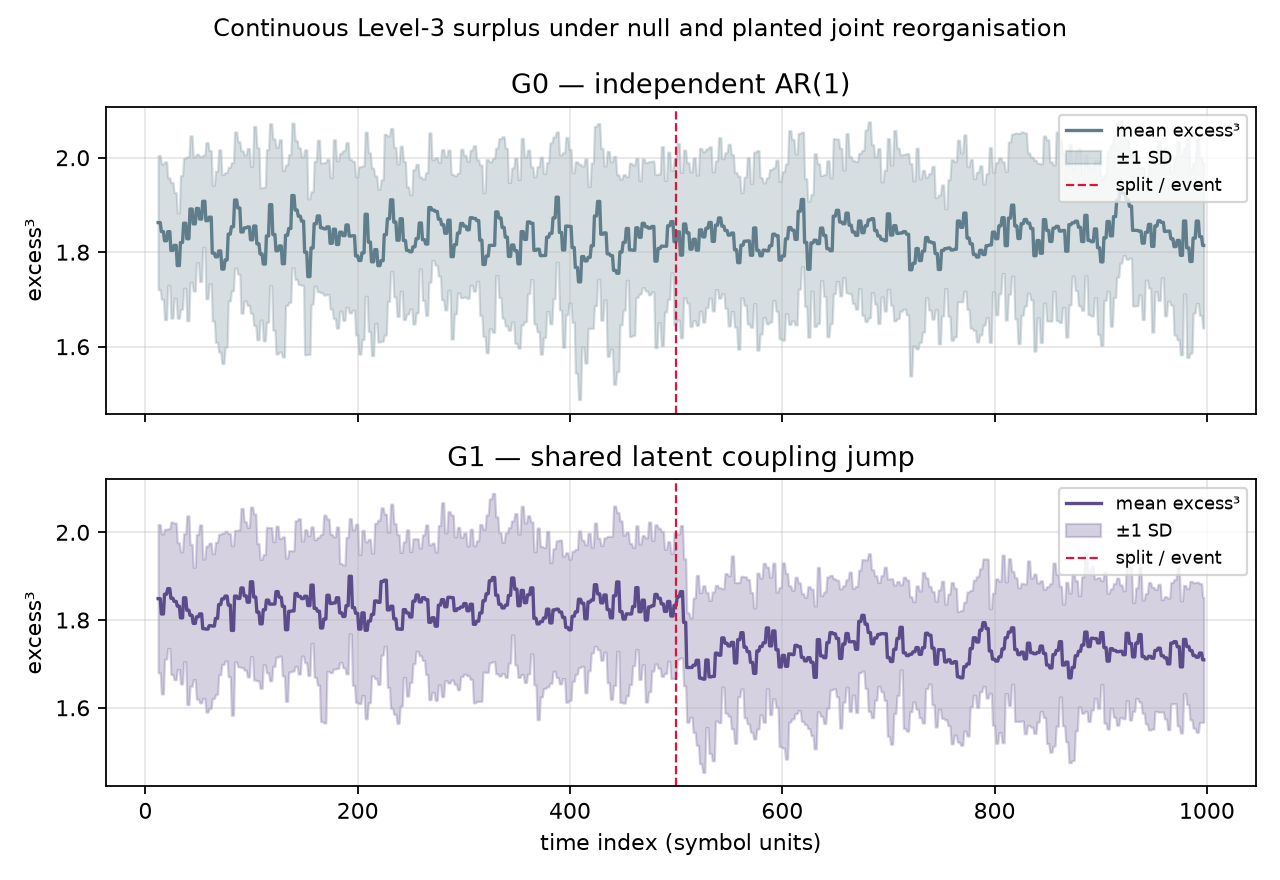
\includegraphics[width=0.95\textwidth]{fig2_g0_g1_trajectories.png}
\caption{Trayectorias de ensamble: media de excess$^3(t)$ $\pm 1$~DE.
L\'inea vertical = evento o corte. \textbf{G0} (casi nulo) permanece plano a
ambos lados del corte. \textbf{G1} (latente compartido) muestra un
desplazamiento post-evento hacia abajo en este generador: el acoplamiento
com\'un infla las parejas y puede reducir el residual Syn. La inferencia no
exige $\Delta>0$; usa $|\Delta|$ a dos colas bajo phase-shuffle. No se
interpreta el signo negativo como ``ausencia de cambio''.}
\label{fig:traj}
\end{figure}

\begin{figure}[H]
\centering
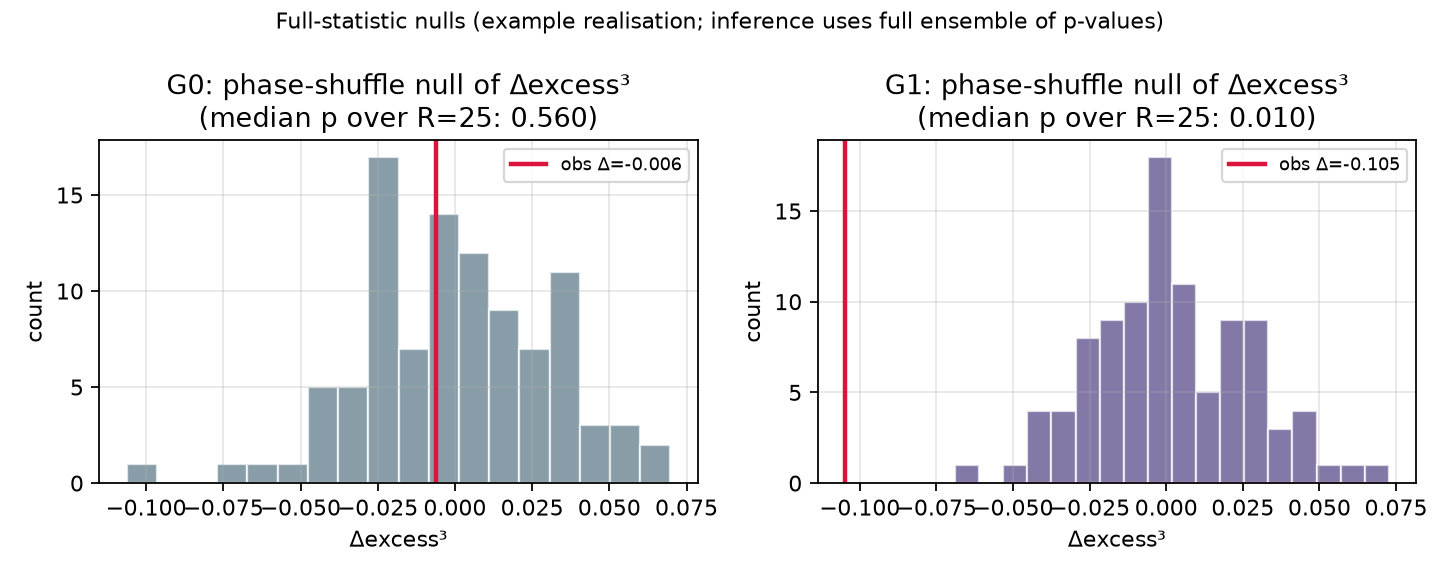
\includegraphics[width=0.95\textwidth]{fig3_nulls_delta.png}
\caption{Nulos de phase-shuffle para $\Delta\mathrm{excess3}$ en una
realizaci\'on ejemplo de G0 y de G1 (valor observado marcado). En G0 el
observado cae en la masa nula; en G1 cae en la cola extrema. Estos paneles
ilustran el mecanismo; el ensamble completo de $p$-valores por realizaci\'on
est\'a en la tabla~\ref{tab:results}. No sustituyen un test reportado solo
como ``media post $>$ media pre''.}
\label{fig:nulls}
\end{figure}

\subsection{Sensibilidad a la ventana y al umbral binario}

La figura~\ref{fig:sens} resume dos sensibilidades. A la izquierda, la media
de $\Delta\mathrm{excess3}$ en funci\'on de la longitud de ventana $w$ para
G0 y G1: la separaci\'on cualitativa se mantiene en un rango moderado de
$w$ (en los paneles de referencia, G0 ronda el cero mientras G1 permanece
desplazado en signo negativo). A la derecha, la ocupaci\'on de $\Phi_3$ en
G1 (pre frente a post) en funci\'on de $\theta_3$. En el umbral de referencia
$\theta_3=0.08$ la ocupaci\'on se satura en pre y post porque el continuo
vive cerca de $O(1)$ en estos generadores. Solo cuando $\theta_3$ se eleva
hacia el grueso de la distribuci\'on continua ($\theta_3\gtrsim 1.2$) aparece
contraste de ocupaci\'on pre/post. Esa figura es el argumento gr\'afico de la
primac\'ia del continuo bajo incertidumbre de umbral: si el relato cient\'ifico
depende solo de tics binarios a un $\theta_3$ bajo, puede no ver lo que el
$\Delta$ continuo ya muestra.

\begin{figure}[H]
\centering
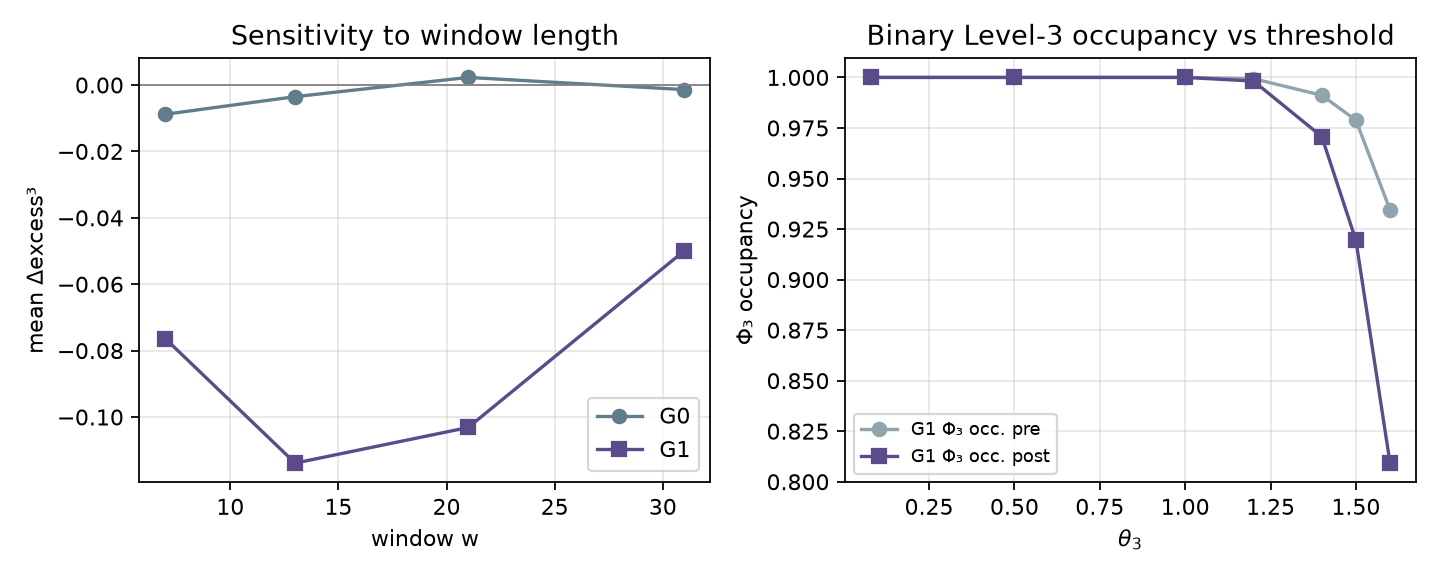
\includegraphics[width=0.95\textwidth]{fig4_sensitivity.png}
\caption{Sensibilidad de ventana y umbral. \textbf{Izquierda:} media de
$\Delta\mathrm{excess3}$ frente a $w$ (G0 $\approx 0$; G1 desplazado en
signo negativo en un rango moderado de $w$). \textbf{Derecha:} ocupaci\'on
de $\Phi_3$ en G1 (pre vs.\ post) frente a $\theta_3$. En el umbral de
referencia $\theta_3=0.08$ (l\'inea discontinua) la ocupaci\'on se
\textbf{satura} porque el continuo vive cerca de $O(1)$: los tics binarios
dejan de discriminar. Solo $\theta_3\gtrsim 1.2$ (cerca del grueso del
continuo) produce contraste de ocupaci\'on. Conclusi\'on operativa: no
construir el relato cient\'ifico solo con $\Phi_3$ a umbral bajo.}
\label{fig:sens}
\end{figure}

La figura~\ref{fig:binary} hace el mismo punto en una sola realizaci\'on de
G1: la traza continua de excess$^3$ lleva el contraste de magnitud, mientras
los tics de $\Phi_3$ dependen del umbral elegido y pueden permanecer
encendidos de forma poco informativa. La figura~\ref{fig:bars} cierra el
panel de resultados con el resumen por brazo: a la izquierda, la media de
$\Delta$; a la derecha, la fracci\'on de realizaciones con $p<0.05$. G1
domina en extremidad; G0 y G2 se agrupan cerca del nulo; G3 queda en una
zona intermedia de especificidad.

\begin{figure}[H]
\centering
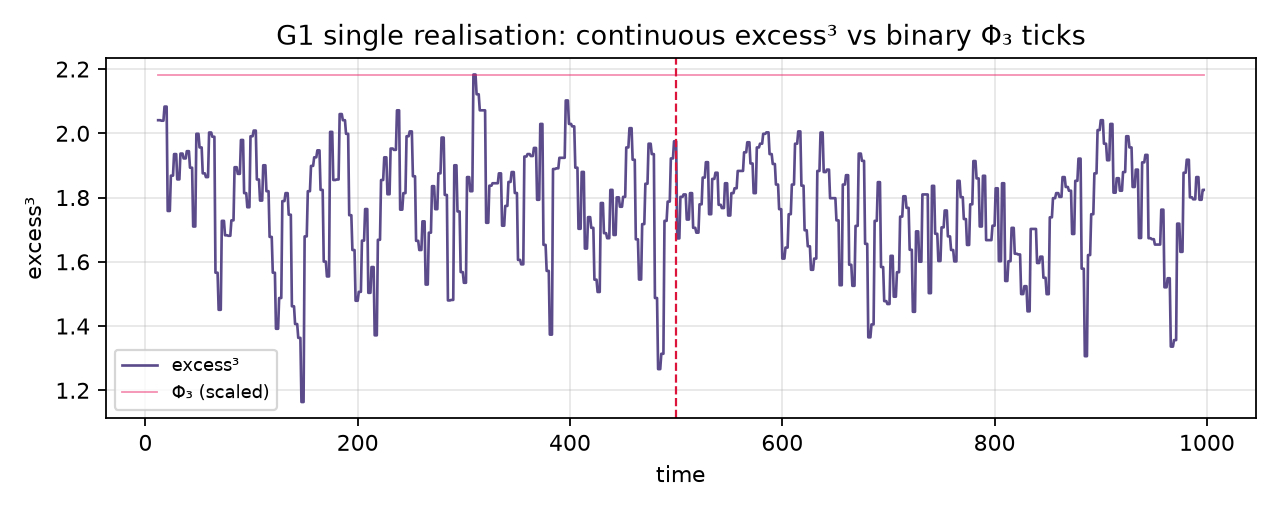
\includegraphics[width=0.92\textwidth]{fig5_continuous_vs_binary.png}
\caption{Una realizaci\'on de G1: excess$^3$ continuo frente a tics de
$\Phi_3$ escalados. La magnitud continua porta el contraste primario; la
ocupaci\'on binaria depende del umbral y puede permanecer ``encendida'' de
forma poco informativa si $\theta_3$ es bajo respecto de la escala del
continuo. L\'imite: un solo trazo no reemplaza el ensamble de la
tabla~\ref{tab:results}.}
\label{fig:binary}
\end{figure}

\begin{figure}[H]
\centering
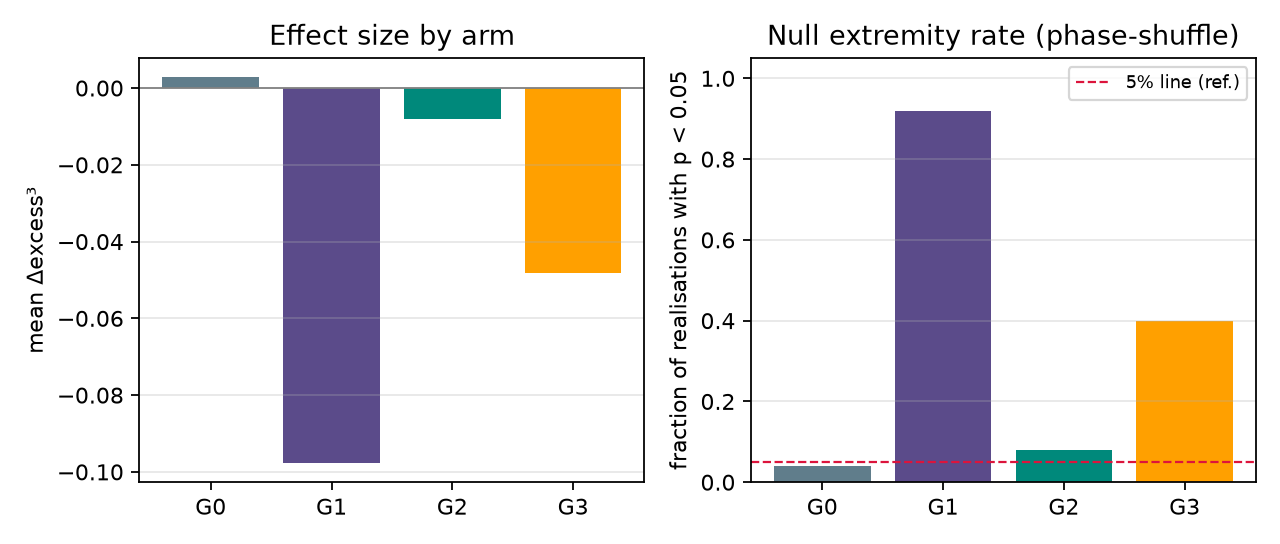
\includegraphics[width=0.92\textwidth]{fig6_arm_summary.png}
\caption{Resumen por brazo del protocolo sint\'etico. \textbf{Izquierda:}
media de $\Delta\mathrm{excess3}$ (G1 m\'as desplazado; G0/G2 cerca de cero;
G3 intermedio). \textbf{Derecha:} fracci\'on de realizaciones con
$p<0.05$ bajo phase-shuffle sobre $|\Delta|$. Lectura leg\'itima:
calibraci\'on direccional bajo generadores controlados. Lectura
ileg\'itima: umbrales num\'ericos universales para datos observacionales.}
\label{fig:bars}
\end{figure}

\subsection{Lectura conjunta de los hallazgos}

Tomados en conjunto, los cuatro brazos y las seis figuras sostienen cuatro
afirmaciones modestas y \'utiles. Primera: bajo un generador casi nulo, el
protocolo de phase-shuffle no fabrica sistem\'aticamente extremidad falsa a
la tasa del $5\%$. Segunda: cuando se planta una reorganizaci\'on conjunta
via latente compartido, $|\Delta\mathrm{excess3}|$ se vuelve extremo en la
gran mayor\'ia de realizaciones. Tercera: el signo de $\Delta$ no debe
forzarse a ser positivo; un aumento de acoplamiento com\'un puede bajar el
residual Syn y producir $\Delta<0$ con $p$ extrema. Cuarta: a umbrales
binarios bajos respecto de la escala del continuo, $\Phi_3$ satura y deja de
discriminar, mientras el continuo sigue haci\'endolo. Ninguna de esas
afirmaciones autoriza a copiar $\theta_3=0.08$ o un corte de $0.15$ bits
como umbral cl\'inico o ecol\'ogico universal.

% =============================================
\section{excess$^3$ en Systemic Tau / RECD}
\label{sec:recd}

En el programa Systemic Tau / RECD, excess$^3$ ocupa el Level~3 de una
jerarqu\'ia ordinal de conjunciones \citep{Padilla2026framework}. Systemic
Tau ($\tau_s$) funciona como un term\'ometro continuo de coherencia
relacional multivariada, construido sobre concordancias de rangos. RECD
funciona como un reloj discreto de eventos ordinales en varios niveles de
profundidad. El nivel 1 se asocia a coincidencias; el nivel 2, a relaciones
de a pares persistentes; el nivel 3, al surplus sin\'ergico, cuya forma
continua es excess$^3$ y cuya forma binaria opcional es $\Phi_3$.

En la implementaci\'on de referencia los niveles se calculan en paralelo. No
existe una implicaci\'on obligatoria del tipo ``si no hay nivel 1, no puede
haber nivel 3'', ni la cadena l\'ogica dura
$\Phi_1\Rightarrow\Phi_2\Rightarrow\Phi_3$ en el c\'odigo. La irreducibilidad
de orden 3 se infiere estad\'isticamente mediante la construcci\'on de excess,
no mediante puertas booleanas (secci\'on~\ref{sec:diseno}). excess$^3$ puede
usarse adem\'as como rasgo de dependencia de orden superior fuera del relato
completo del reloj RECD.

% =============================================
\section{Usos por dominio}
\label{sec:dominios}

Las vi\~netas que siguen son marcos de pregunta y de lenguaje, no resultados
emp\'iricos de un dataset concreto. En ecolog\'ia, la pregunta natural es si
tres indicadores de estado de un ecosistema reorganizan su c\'odigo ordinal
conjunto antes de un cambio de r\'egimen, aunque ninguno dispare por s\'i
solo un early-warning cl\'asico basado en varianza o autocorrelaci\'on
lag-1. excess$^3$ puede actuar entonces como complemento relacional de esas
herramientas univariadas \citep{Scheffer2009}, siempre vigilando la
estacionalidad y otros conductores comunes que inflan parejas.

En epidemiolog\'ia y salud ambiental, la pregunta an\'aloga involucra clima,
vector e incidencia alrededor de un brote. excess$^3$ no identifica qu\'e
variable causa los casos; se\~nala una reorganizaci\'on conjunta que puede
merecer seguimiento mecan\'istico. En fisiolog\'ia y cuidado cr\'itico, el
inter\'es recae en si los patrones ordinales cardiorrespiratorios cambian su
surplus conjunto cerca de una ventana de descompensaci\'on; all\'i la
primac\'ia del continuo es especialmente relevante. En ciencias del clima,
tres \'indices regionales pueden exhibir estructura residual m\'as all\'a del
mapa de teleconexiones de a pares cerca de un posible elemento de
basculaci\'on. En neurociencia y cognici\'on, donde el lenguaje PID es
frecuente, conviene declarar que excess$^3$ es un proxy vecino del \'atomo
sin\'ergico y no el lattice completo \citep{Williams2010,Rosas2019}. En
sistemas sociales o econ\'omicos, los shocks comunes tienden a inflar
parejas; un $\Delta$ negativo tras una sincronizaci\'on masiva puede ser
exactamente la geometr\'ia del conductor com\'un, en la misma l\'inea del
brazo G1.

% =============================================
\section{Flujo de an\'alisis recomendado}
\label{sec:flujo}

Un uso disciplinado de excess$^3$ comienza por formular el contraste
cient\'ifico antes de inspeccionar $p$-valores. Los tres canales se eligen
con una hip\'otesis conjunta expl\'icita. Los par\'ametros de codificaci\'on se
fijan a priori. Se calcula la curva continua y el $\Delta$ pre-especificado,
y se eval\'ua un nulo adecuado ---por ejemplo phase-shuffle--- sobre ese
mismo estad\'istico. La inspecci\'on de Syn y Surp por separado aclara qu\'e
componente se mueve. Las curvas continuas se reportan como lectura
primaria; $\Phi_3$ queda como discretizaci\'on secundaria, acompa\~nada de
comprobaciones de saturaci\'on si se usa. El lenguaje de resultados se
mantiene operativo ---dependencia, reorganizaci\'on, surplus--- y evita
causa o emergencia demostrada. Cuando el tama\~no muestral lo permite, se
incluye al menos una sensibilidad, por ejemplo otra ventana o otro $m$.
Los estimadores y el software se alinean con
\citep{Padilla2026excess3}.

Un manuscrito o informe deber\'ia dejar constancia, como m\'inimo, de $T$,
$N$, la tasa de muestreo, $(m,\tau)$, $w$, los pesos $(0.6,0.4)$ con la
declaraci\'on de que no se retocaron sobre el dataset de la hip\'otesis, el
estad\'istico primario continuo, $\theta_3$ solo si se usa $\Phi_3$, el
modelo nulo con su n\'umero de surrogados y la regla a una o dos colas, la
versi\'on de software cuando exista, y las no-afirmaciones de no causalidad
y de no PID completo.

% =============================================
\section{Seis decisiones de dise\~no}
\label{sec:diseno}

Las seis respuestas siguientes condensan contratos metodol\'ogicos que, si
solo aparecen como notas al margen, se malinterpretan con facilidad en
informes aplicados. No son matizaciones posteriores: son elecciones fijas
del proxy de Level~3 \citep{Padilla2026excess3}.

\paragraph{Por qu\'e $0.6/0.4$.}
Los pesos h\'ibridos
$(\alpha_{\mathrm{Syn}},\alpha_{\mathrm{Surp}})=(0.6,0.4)$ son
\textbf{constantes heur\'isticas fijas a priori}. Expresan una preferencia
moderada por el residual multiinformacional frente a la sorpresa de
independencia, pero \emph{no} se estiman por validaci\'on cruzada, b\'usqueda
en malla ni ning\'un otro optimizador sobre el dataset cient\'ifico bajo
prueba. La pre-especificaci\'on preserva la falsabilidad: excess$^3$
permanece un estad\'istico de prueba declarado y no un descriptor
post~hoc que pueda retocarse hasta obtener el $p$-valor deseado.
Pares de pesos alternativos son admisibles solo si se registran antes de
mirar los datos de la hip\'otesis; reponderar en silencio no lo es.

\paragraph{Syn frente a Surp.}
$\mathrm{Syn}=[\mathrm{TC}-I_{\mathrm{pair}}]_+$ es el residual no negativo
de la correlaci\'on total despu\'es de restar una baseline de informaci\'on
mutua de orden~2: pregunta cu\'anta organizaci\'on multiinformacional
permanece una vez que la estructura de a pares ha sido restada.
$\mathrm{Surp}$ es otra geometr\'ia: punt\'ua las tuplas de s\'imbolos
conjuntos que son m\'as frecuentes de lo que permitir\'ia la independencia
completa ($p_{\mathrm{obs}}$ frente a $\prod_i p_i$), reteniendo solo las
contribuciones de log-raz\'on positivas. El h\'ibrido mantiene visibles
ambas lentes en lugar de colapsarlas en un solo \'atomo
(secciones~\ref{sec:entropia}--\ref{sec:piezas}).

\paragraph{excess$^3$ frente a $\Phi_3$.}
El continuo $\mathrm{excess3}(t)$ es la magnitud \textbf{primaria} de
Level~3: las trayectorias, los gradientes y los contrastes
$\Delta\mathrm{excess3}$ viven en la escala continua. El binario
$\Phi_3=\mathbf{1}\{\mathrm{excess3}>\theta_3\}$ existe solo para conteos
de tics, pantallas tipo r\'aster y res\'umenes de tasa. La ocupaci\'on de
$\Phi_3$ puede saturar cuando $\theta_3$ queda por debajo del grueso de la
distribuci\'on continua; esa saturaci\'on es propiedad del umbral, no
evidencia de que el Level~3 carezca de se\~nal
(secciones~\ref{sec:leer},~\ref{sec:validation}).

\paragraph{No es PID completo.}
excess$^3$ es un \textbf{proxy computable} de surplus sin\'ergico de orden~3.
No es una descomposici\'on parcial de informaci\'on completa: no a\'isla
\'atomos \'unicos, redundantes y sin\'ergicos de un lattice PID
\citep{Williams2010,Bertschinger2014}. La extensi\'on te\'orica natural
consiste en sustituir la f\'ormula h\'ibrida por un \'atomo de sinergia PID
estable cuando el tama\~no muestral y la calidad del estimador lo permitan;
mientras tanto, el h\'ibrido es el contrato operativo de Level~3
(secci\'on~\ref{sec:noes}).

\paragraph{Modelo nulo.}
La inferencia se dirige al \textbf{contraste completo declarado} ---por
regla general $|\Delta\mathrm{excess3}|$ bajo un Monte Carlo a dos
colas--- y no a una comparaci\'on vaga de medias contra medias de medias.
El surrogado por defecto es el barajado de fase independiente (u otro que
preserve la estructura univariada relevante y rompa la dependencia
cruzada entre canales). El protocolo consiste en situar $T_{\mathrm{obs}}$
dentro de la nube $\{T^{(b)}\}$; contrastar solo promedios de promedios
es un anti-patr\'on (secci\'on~\ref{sec:nulos}).

\paragraph{Anidamiento operativo.}
En el lenguaje de RECD puede hablarse de niveles m\'as profundos como
afirmaciones m\'as fuertes. En el software, $\Phi_1$, $\Phi_2$ y
excess$^3$/$\Phi_3$ se calculan \textbf{en paralelo} a partir de la misma
ventana simb\'olica $S_t$. No existe implicaci\'on l\'ogica dura
$\Phi_1\Rightarrow\Phi_2\Rightarrow\Phi_3$ en el c\'odigo de referencia. La
irreducibilidad de orden~3 se infiere \emph{estad\'isticamente} mediante la
construcci\'on de excess (Syn tras baseline de parejas, m\'as Surp), no
forzando una cadena de puertas booleanas (secci\'on~\ref{sec:recd}).

% =============================================
\section{Preguntas frecuentes complementarias}
\label{sec:faq}

Adem\'as de las seis decisiones de la secci\'on~\ref{sec:diseno}, conviene
cerrar tres confusiones habituales. Leer un excess$^3$ alto como
demostraci\'on de emergencia es ileg\'itimo: lo que hay es se\~nal de
organizaci\'on residual bajo un c\'odigo concreto. Un $\Delta$ negativo no
implica fracaso: en G1 es el patr\'on esperado bajo absorci\'on por parejas,
y se interpreta inspeccionando Syn frente a Surp y la extremidad de
$|\Delta|$ bajo el nulo. No es necesario adoptar el marco RECD completo
para emplear excess$^3$: bastan definici\'on operativa, nulo e
interpretaci\'on contextual. Con muestras peque\~nas el estimador sale con
facilidad de su zona confiable. Por \'ultimo, excess$^3$ no reemplaza los
early-warnings cl\'asicos basados en varianza o memoria univariada; los
complementa cuando la hip\'otesis es relacional \citep{Scheffer2009}.

% =============================================
\section{Ejemplo de redacci\'on de resultados}
\label{sec:narracion}

Plantilla lista para adaptar (contraste alineado con el brazo G1 de
referencia: media pre $\GonePre$, post $\GonePost$,
$\Delta=\GoneDelta$, mediana $p=\GoneMedP$ sobre $|\Delta|$ en el ensamble).

\paragraph{Modelo de p\'arrafo (leg\'itimo).}
\begin{quote}
\small\raggedright
``Bajo hiperpar\'ametros pre-especificados ($m{=}3$, $w{=}13$, pesos
$0.6/0.4$), el contraste $\Delta\mathrm{excess3}$ fue $\GoneDelta$
(medias pre/post $\GonePre$/$\GonePost$).
La extremidad de $|\Delta|$ bajo surrogados de barajado de fase
independiente por canal alcanz\'o mediana $p=\GoneMedP$ en el ensamble de
referencia.
La inspecci\'on de componentes es coherente con un aumento de la
dependencia de a pares tras el evento, que reduce el residual
$\mathrm{Syn}$.
Interpretamos el cambio como reorganizaci\'on hacia acoplamiento m\'as
compartido, no como ausencia de se\~nal.
Reportamos la curva continua como lectura primaria; la ocupaci\'on de
$\Phi_3$ a $\theta_3{=}0.08$ no se usa como \'unica evidencia.''
\end{quote}

\paragraph{Frases prohibidas (y por qu\'e).}
\begin{itemize}[leftmargin=*,itemsep=2pt]
  \item ``La sinergia baj\'o; el sistema perdi\'o integraci\'on'' --- convierte
  un signo en tesis de colapso y omite la baseline de parejas.
  \item ``Demostramos causalidad / emergencia'' --- excess$^3$ mide
  dependencia residual bajo un c\'odigo, no mecanismo.
  \item ``$\Phi_3$ prueba Level~3'' --- el binario es secundario; a umbral
  bajo puede saturarse.
  \item ``Como $\Phi_1$ y $\Phi_2$ activaron, $\Phi_3$ debi\'o activar'' ---
  el anidamiento RECD es paralelo, no implicaci\'on booleana.
  \item ``Optimizamos $0.6/0.4$ en estos datos'' --- rompe la
  falsabilidad del contrato (secci\'on~\ref{sec:diseno}).
\end{itemize}

% =============================================
\section{Referencias de m\'etodos y marco}
\label{sec:mapa}

La especificaci\'on can\'onica de excess$^3$, el protocolo de nulos y la
validaci\'on sint\'etica completa se desarrollan en
\citep{Padilla2026excess3}. El contexto de Systemic Tau y RECD aparece en
\citep{Padilla2026framework}. La codificaci\'on ordinal de Bandt--Pompe se
debe a \citep{BandtPompe2002}. Los early-warnings cl\'asicos se revisan en
\citep{Scheffer2009}. El vecindario te\'orico de PID y de las medidas
globales de sinergia y redundancia puede abordarse desde
\citep{Williams2010,Rosas2019,Timme2018}.

% =============================================
\section{S\'intesis}
\label{sec:bolsillo}

excess$^3$ responde a una pregunta acotada: si, en una ventana de s\'imbolos
ordinales, hay organizaci\'on de tr\'io m\'as all\'a de lo que ya cuentan las
parejas y m\'as all\'a de lo que permitir\'ia la independencia completa. La
correlaci\'on total resume la organizaci\'on conjunta; la baseline de parejas
estima lo ya visible de a dos; $\mathrm{Syn}$ retiene el sobrante no
negativo; $\mathrm{Surp}$ retiene la sorpresa de co-ocurrencia; y la
combinaci\'on fija $0.6\,\mathrm{Syn}+0.4\,\mathrm{Surp}$ produce el
puntaje continuo. Los pesos no se retocan sobre el dataset de la hip\'otesis.
La lectura primaria es la curva y el contraste $\Delta$; el binario
$\Phi_3$ es secundario. La inferencia va sobre el estad\'istico completo
(p.\,ej.\ $|\Delta\mathrm{excess3}|$) con un nulo que rompe dependencia
cruzada; el anidamiento RECD es operativo y paralelo, no una implicaci\'on
booleana; y el objeto no es un lattice PID completo, sino un proxy cuya
extensi\'on natural es el \'atomo de sinergia cuando el estimador lo permita
(secci\'on~\ref{sec:diseno}). La validaci\'on sint\'etica muestra nulo bien
comportado en G0, extremidad alta en G1 con $\Delta$ potencialmente
negativo, casi-nulo en G2 bajo este dise\~no, intermedio en G3, y saturaci\'on
de $\Phi_3$ a umbrales bajos. El lenguaje leg\'itimo es el de la dependencia
y el surplus, no el de la causa demostrada ni el de la emergencia
metaf\'isica.

% =============================================
\section{Glosario}
\label{sec:glosario}

\begin{description}[style=nextline,leftmargin=1em,itemsep=5pt]
  \item[Dependencia estad\'istica]
    Relaci\'on por la cual el conocimiento de una variable reduce la
    incertidumbre sobre otra bajo un estimador dado; no implica causaci\'on.

  \item[Entrop\'ia]
    Medida de incertidumbre o impredecibilidad de una variable.

  \item[Informaci\'on mutua]
    Informaci\'on compartida entre \emph{dos} variables; se anula bajo
    independencia.

  \item[Orden 3]
    Estructura estad\'istica que involucra tres variables a la vez y no se
    agota en las relaciones de a pares.

  \item[Proxy]
    Medida pr\'actica que se aproxima a un concepto ideal ---aqu\'i, el
    surplus sin\'ergico--- sin coincidir necesariamente con su definici\'on
    m\'as pura.

  \item[Phase-shuffle]
    Surrogado que randomiza la fase de cada canal en Fourier, conservando
    buena parte del espectro y rompiendo organizaci\'on cruzada fina.

  \item[Redundancia (informal)]
    Situaci\'on en la que varias variables repiten informaci\'on parecida,
    t\'ipicamente por un conductor com\'un.

  \item[Sinergia (informal)]
    Situaci\'on en la que el conjunto informa de un modo que las partes,
    separadas, no logran.

  \item[Surrogado / nulo]
    Datos artificiales que conservan algunos rasgos del proceso y rompen
    otros, para evaluar si un contraste observado podr\'ia producirse sin la
    organizaci\'on cruzada de inter\'es.

  \item[Ventana]
    Segmento local de tiempo sobre el que se estiman entrop\'ias, residuales
    y excess$^3$.

  \item[Baseline de parejas ($I_{\mathrm{pair}}$)]
    Escala de informaci\'on mutua media de a dos, usada para restar de la
    multiinformaci\'on lo ya visible sin mirar el tr\'io completo.

  \item[Contraste $\Delta\mathrm{excess3}$]
    Diferencia de medias de excess$^3$ entre dos reg\'imenes (p.\,ej.\ post
    menos pre); estad\'istico habitual sobre el que se aplica el nulo.

  \item[Ocupancia de $\Phi_3$]
    Fracci\'on de ventanas (o de tiempo) en las que
    $\mathrm{excess3}>\theta_3$. Secundaria respecto del continuo; a
    umbrales bajos puede saturarse y dejar de discriminar.

  \item[Anidamiento paralelo]
    C\'alculo simult\'aneo de $\Phi_1$, $\Phi_2$ y excess$^3$/$\Phi_3$ sobre
    la misma ventana simb\'olica, \emph{sin} forzar
    $\Phi_1\Rightarrow\Phi_2\Rightarrow\Phi_3$ en el software de referencia.
\end{description}

% =============================================
\section*{Disponibilidad de datos y c\'odigo}
\addcontentsline{toc}{section}{Disponibilidad de datos y c\'odigo}

Las fuentes de la familia (m\'etodos, esta introducci\'on y la gu\'ia en
ingl\'es), las figuras y los resultados de ensamble est\'an en el repositorio
compartido
\href{\ExcessThreeRepo}{\ExcessThreeRepoShort}
(carpetas \texttt{methods/}, \texttt{intro/}, \texttt{primer/}).
El DOI de archivo se a\~nadir\'a en el release de Zenodo.
La implementaci\'on de referencia Level~3 coincide con el stack abierto
\texttt{systemictau} \citep{Padilla2026software}
(\url{https://doi.org/10.5281/zenodo.20576241}). Este documento no redefine
el estimador: para ecuaciones, nulos y checklist de reporte, c\'itese
\citep{Padilla2026excess3}.

\section*{Financiaci\'on y conflictos}
\addcontentsline{toc}{section}{Financiaci\'on y conflictos}

Sin subvenci\'on externa dedicada a este preprint. El autor declara no tener
conflictos de inter\'es.

\section*{Licencia}
\addcontentsline{toc}{section}{Licencia}

Se prev\'e distribuci\'on bajo Creative Commons Attribution 4.0 International
(CC~BY~4.0) al depositarse en abierto, salvo requisito distinto del
repositorio o revista.

\section*{Agradecimientos}
\addcontentsline{toc}{section}{Agradecimientos}

Los errores de exposici\'on o de interpretaci\'on son responsabilidad del
autor.

% =============================================
\bibliographystyle{plainnat}
\bibliography{references}

\end{document}
